%==============================================================================================================================
% methods.tex : DESCRIBES THE MODEL AND ANALYZES USED
%=============================================================================================================================
\chapter{Methods}
\label{experiment_chapter}
%------------------------------------------------------------------------------

\section{Modeling }
\subsection{Configuration}
% -- ROMS --%
ROMS is a three-dimension, free-surface, terrain-following numerical model that solves the Reynolds-averaged (time-averaged) Navier-Stokes equations using the hydrostatic 
and Boussinesq assumptions. The hydrostatic assumption assumes the vertical pressure force is balanced by the weight of the fluid parcel. In which case, the pressure at a given  
depth is given by the hydrostatic equation, $\frac{\partial P}{dz}=-\rho g$. The Boussinesq approximation assumes that density variations are negligible in the Navier-Stokes 
equations, except for the buoyancy term where $\rho$ is multiplied by $g$.  The non-linear equations of motion are solved using  a predictor(leap-frog)-corrector(Adam-Molten) 
finite difference scheme. To solely look at the affects of surface stress and stratification on near-inertial energy the
model was configured for no radiative forcing. Without radiative forcing the heat content of the water column can not change and stratification can not form on its own.  

Lake Superior was modeled as closed basin with no inflows or outflows. The bathymetry used has a spatial resolution of 2km \citep{schwab1996computerized} and was
smoothed with the following three point moving average : 

% -- THREE POINT MOVING AVERAGE
\begin{equation}
	x_t = 0.25 x_{t-1} + 0.5 x_t + 0.25 x_{t+1} 
\end{equation}
until the Beckman and Haidvogel number  was less than 0.4. A small Beckman and Haidvogel number ensure model stability and avoids spurious deep water currents. 
This number is defined as : 

% -- BECKMAN AND HAIDVOGEL NUMBER
\begin{equation}
	R_x=\max \frac{| h(i)-h(j) |}{h(i)+h(j)}
\end{equation}
where $h(i)$ and $h(j)$ is the depth at neighboring grid cells and $R_x$ is the Beckman and Haidvogel number.

Lake Superior spans about 2.5 degrees of latitude, the Coriolis parameter over this range changes by about 3\%. Because the change in the Coriolis parameter is small the model
configured using an f-plane approximation. The Mellor-Yamada closure scheme was used in the model, which takes eddy viscosity into account and estimates turbulence 
on scales which can not be resolved by the model. Model output was  linearly interpolated onto a common grid. One implication of this is current velocities one grid cell away from the coast
must be discarded since the interpolation used points outside the basin. A diagram of a grid cell is provided below. 

% -- ROMS GRID CELL
\FIGURE{4}{grid_cell.pdf}{Arakawa-C Grid Cell}{The Arakawa-C grid cell computes density, depth, and Coriolis frequency at the center of each cell. The $u$ and $v$ 
component of the velocity are computed half a cell distance away. $\Delta \eta$ and $\Delta \zeta$ are the resolution of the model in the meridional and zonal direction respectively.}

The model used a time step of $\Delta t = $200 seconds and data was output hourly.  The time step at the surface is $\frac{\Delta t}{30}$, since the waves evolve much faster at the surface. 
For stability, the CFL (Courant-Friedrichs-Lewy) condition requires the  courant number to be less than 1 everywhere in the model. This condition can be expressed as
 $|\frac{V\Delta t}{\Delta x}| \le 1$, where $V$ is the maximum internal wave speed $\Delta t$ is the internal time step  and $\Delta x$ is the horizontal spatial resolution. 
 It is easy to show the CFL condition holds at the deepest point in the model (350 m) by calculating the courant number for a wave at the surface and at the internal interface. 

% -- CALCULATING COURANT NUMBERS
\begin{equation*}
\begin{aligned}[c]
\text{\bf External Courant } &  \text{ \bf Number} \\
	\frac{V_{external} \frac{\Delta t}{30}}{\Delta x} & \\
	\frac{\sqrt{gH_{max}} \frac{\Delta t}{30}}{\Delta x} & \\
	\frac{\sqrt{9.8 ms^{-1} 350m} \frac{200 s}{30}}{2000m} & \\
	0.20 & < 1
\end{aligned}
\qquad\ \qquad
\begin{aligned}[c]
\text{\bf Internal Courtant} &  \text{ \bf Number}  \\
	\frac{V_{internal}\Delta t}{\Delta x} & \\
	\frac{\sqrt{g^{\prime}h^{\prime}}\Delta t}{\Delta x} & \\
	\frac{\sqrt{9.8*0.001*\frac{20m * 330m}{350m}} * 200 s}{2000m} & \\
	0.04 & < 1
\end{aligned}
\end{equation*}

The model is likely to be stable since the courant number is always less than one. The purpose of the CFL condition is so we do not advect material through a grid cell
in the given time step. Note that the CFL condition is required for model stability but is not sufficient and therefore will not guarantee a stable model. More information
on model stability can be found in \citet{glover_modeling_methods}.

%====================================================================================================================================
% -- VERTICAL STRUCTURE
%===================================================================================================================================
\subsection{Vertical Structure}

The model was configured with 30 vertical layers staggered throughout the water column. The spacing between vertical levels varied from 0.2 m at the surface
to 15 m at the bottom. The vertical stretching was given by : 

% -- STRETCHING PARAMETER
\begin{equation} 
	C(\sigma)=\frac{1-\cosh(\theta_s \sigma)}{\cosh(\theta_s) -1} 
\end{equation}
where $\theta_s=3$,  $\sigma=\frac{k-N-0.5}{N}\text{\ \ \ } k=1\ldots N$, where $N$ is the number of vertical layers. 

Two types of thermal structures were used, a homogenous water column of uniform temperature and a stratified water column. The 
well mixed water column was chosen to be 4$^{\circ}C$ since it is close to $T_{md}$. However, it should be noted that any temperature could have been chosen and this 
temperature does affect the dynamics of the water column. Stratification was modeled as a two layer system, the modeled thermal structure was given by the following equation. 

% -- THERMAL STRUCTURE
\begin{equation} 
	T(z)=T_{bot}+(\frac{T_{top}-T_{bot}}{2})*(1+\tanh(\frac{(z+z_{cline})}{s}))
\end{equation}
Where $T_{bot}$ is the temperature of the bottom layer, $T_{top}$ is the temperature of the top layer, $z_{cline}$ is the thermocline depth, and $s$ 
is a steepness parameter for the gradient of the thermocline. The following values were used in the thermal structure equation. 



%==================================================================================================================
% -- DEFINITION OF TERMS
\begin{table}[H]
	\centering
		\caption{Thermal Stratification Values }
		\vspace{6pt} 
	\label{table:stratVals} % is used to refer this table in the text 
	\begin{tabular}{c c c}
	\hline \hline 									%inserts double horizontal lines 
	\textbf{Parameter} & \textbf{Value} & \textbf{Description} \\ [0.5ex] % inserts table 
	%--------------------------------------------------------------------------------------------------------------------------------------
	% -- BODY OF THE TABLE
	\hline 										
	$T_{bot}$ & 4$^{\circ}C$ & Bottom layer temperature  \\ 	
	$T_{top}$ & 21 $^{\circ}C$ & Top layer temperature \\ 
	$z_{cline}$ & 20 m & Thermocline depth  \\ 
	$s$ & 2 & Thermocline steepness parameter  \\ [1ex] 	% [1ex] adds vertical space 
	\hline 
	\end{tabular}		
\end{table}
%==================================================================================================================

A diagram of the initial thermal structure is shown below for a point in the model which has a depth of 160m.

% -- INITIAL THERMAL STRUCTURE
\FIGURE{4}{ROMS_initial_thermal.pdf}{Modeled Initial Thermal Structure}{Shows the initial thermal structure for a point where the max depth is 160m. 
This also shows the spacing in the model.}
The spacing between grid cells decreases with depth. The spacing at the top is on the order of a meter while at the bottom it is on the order of 20 m. One downside to
this thermal structure is only about three or four temperature readings are taken in the metalimnion so the thermocline can not be highly resolved.

%===================================================================================================================================
% -- FORCING -- %
%=============================================================================================================================
\subsection{Forcing}

Two types of forcing were used, an impulse of idealized wind stress and temporally and spatially varying wind stress. The idealized forcing was a spatially 
uniform pulse of wind stress with a  magnitude of 0.1 $N m^{-2}$;  this is equivalent to a wind speed of $8\ ms^{-1}$ at 10m above the surface  \citep{fairall1996bulk}. 
 To maximize the energy input at the inertial frequency the duration of the wind pulse lasted for half an inertial period \citep{boyce1989thermal}.

Temporally and spatially varying wind stress was derived from the North American Regional Reanalysis (NARR) climatology data. This is an extension of NCEP Global
Reanalysis which runs models of the North American region. NARR provides high resolution (32km spatial / 45 layers) climatology model output from 1979 up to today 
with a temporal resolution of 3 hours. The zonal and meridional wind speeds at 10m above the surface from 2011 were used to compute the wind stress at  the surface. 
The modeled wind stress was linearly interpolated to an hourly time grid and objective analysis was used to interpolate the output onto a 2km x 2km grid. 
To show the spatial variability in the wind stress snapshots of the wind stress derived from NARR climatology output are provided below.

% -- NARR WIND STRESS -- %
% \FIGURE{size}{figure name in Figures dir.}{caption}{label}
\FIGURE{4}{NARR_stress.pdf}{NARR Stress}{Snapshots of the wind stress}

The surface stress computed from NARR was compared to wind stress computed from observed NDBC data.
The NDBC wind stress appears coherent at the core mooring sites, however, the NARR stress does not completely capture all the features of the observed stress. 
There are also times when the two series are 180$^\circ$ out of phase. Plots of observed and modeled wind stress are provided below. 

% -- COMPARE WIND STRESS -- %
% \FIGURE{size}{figure name in Figures dir.}{caption}{label}
%\FIGURE{2.5}{compare_wind_stress.pdf}{Compare Wind Stress}{Compares observed wind stress at the core mooring
%sites to wind stress comported from NARR.}

A comparison between each site is given below. The NARR stress follows the general shape of the observed
NDBC stress but acts as a smoothed version of the observed data. In other words, the NARR stress does not follow
of the extreme events. 

% -- CORE MOORING STRESS-- %
% \FIGURE{size}{figure name in Figures dir.}{caption}{label}
%\FIGURE{2.5}{core_mooring_stress.pdf}{Core Mooring Stress}{Compares observed wind stress at the core mooring sites to wind stress comported from NARR. 
%The black line is observed NDBC data at each mooring and the dotted red line is the modeled stress from NARR}
\FIGURE{2.5}{NDBC_NARR_direction.pdf}{Core Mooring Stress}{Compares observed wind stress at the core mooring sites to wind stress computed from NARR. 
The black arrow represents the observed (NDBC) data and the red arrows represent the NARR stress.}

% -- NDBC vs NARR - %
% \FIGURE{size}{figure name in Figures dir.}{caption}{label}
\FIGURE{2}{NDBC_vs_NARR.pdf}{NDBC vs NARR}{Wind stress derived from NDBC vs wind stress derived from NARR at each mooring location.}
%======================================================================================================================================
% --COMPUTATION -- %
%======================================================================================================================================
\subsection{Computation}

Computation was done at the Minnesota Supercomputing Institute (MSI) located on the Twin Cities campus of the University of Minnesota. 
The model was partitioned into 16 equal pieces each computed on different computing nodes on MSI's Calhoun cluster.  Calhoun is an SGI Altix XE 1300 Linux cluster 
with 180 SGI Altix XE 300 computing nodes. Each node contains two quad-core 2.66 GHz Intel Xeon processors sharing 16 GB of memory.
In total, Calhoun consists of 1440 computing cores and 2.8 TiB of main memory. A model run of 90 days  and outputting every hour would takes approximately 16 hours
to complete using 16 processors. 

%%%%%%%%%%%%%%%%%%%%%%%%%%%
% LAKE SUPERIOR MOORING ARRAY
%%%%%%%%%%%%%%%%%%%%%%%%%%%
\section{Lake Superior Mooring Array}
% -- MOORING ARRAY
The Lake Superior mooring array is a collection of up to seven moorings which have been continuously deployed since 2005. 
In 2005 the Western Mooring (WM) was deployed and was the only mooring for three years. The Eastern (EM) and Central (CM) Moorings
were included in the array in 2008. These three moorings form the "core mooring" array which is still in operation today. 
The core moorings locations were chosen to be with 1 to 2 km of National Data Buoy Center (NDBC) buoys. with the WM, CM, and EM 
locations coinciding with NDBC buoys 45006, 45001, and 45004, respectively. To increase spatial variability four more moorings have included, 
these are the Far Western (FWM); Northern (NM); Southern (SM); and  Far Eastern Moorings (FEM). 
However, these supplemental moorings were only in operation from 2008 to 2012. 
The moorings remain in continuous operation once deployed but are removed once or twice a year to replace batteries and retrieve data. 

Instruments on the moorings have included thermistor strings, Acoustic Doppler Current Profilers (ADCP) \citep{bugnon_1991}, ice profilers, $O_2$ sensors, 
$NO_3$ sensors, and sediments traps. However, this thesis will only discuss thermistor and ADCP data sets. 

Each mooring is equipped with 10 to 13 thermistors irregularly spaced throughout the water column. Thermistors are spaced closer together near
the surface to capture the abrupt temperature change in the thermocline during the stratified season and coarsely spaced near the bottom 
where the temperature remains relatively constant throughout the year. Due to coast guard restrictions, thermistors extend 7 to 10 meters below the water surface. 
The coincident NDBC buoy can be used to fill in the temperature gap near the surface, since they record temperature at 1 m depth. 
The anchor and acoustic release limit the bottom thermistor to a depth of 3 to m meters above the lake bed. 

A few different thermistor models have included on the moorings, including Brancker Research (RBR) TR-1000, TR-1050, TR-1060, and TD-2050 sensors, 
and Seabird Electronics SBE-39 and SBE-39P sensors. Each thermidor is deployed with a pressure sensor to verify the depth. The storage capacity 
of the instruments limits the sampling rate, with the TR-1000 and SBE sensors taking measurements every 10 minutes, and the TR-1050, TR-1060, 
and TD-2050 sensors taking measurements every 1 minute


% -- LAKE SUPERIOR MOORING ARRAY LOCATIONS -- %
% \FIGURE{size}{figure name in Figures dir.}{caption}{label}
\FIGURE{2.5}{mooring_array.pdf}{Lake Superior Mooring Array}{Locations of active and inactive moorings in Lake Superior deployed since 2005}


%==================================================================================================================
% -- MOORING ARRAY
\begin{table}[H]
	\centering
		\caption{Mooring Array }
		\vspace{6pt} 
	\label{table:stratVals} % is used to refer this table in the text 
	\begin{tabular}{c c c c}
	\hline \hline 									%inserts double horizontal lines 
	\textbf{Mooring Name} & \textbf{Latitude} & \textbf{Longtidue} & \textbf{Depth (m)} \\ [0.5ex] % inserts table 
	%--------------------------------------------------------------------------------------------------------------------------------------
	% -- BODY OF THE TABLE
	\hline 										
	Western Mooring (WM) & 47$^{\circ}$ 19.018' & 89$^{\circ}$ 48.520' & 185 \\ 
	Central Mooring (CM)   & 48$^{\circ}$ 1.384' & 87$^{\circ}$ 46.006' & 255 \\ 
	Eastern Mooring (EM)       & 47$^{\circ}$ 32.186' & 86$^{\circ}$ 34.261' & 213 \\ 
	\hline
	Far Western Mooring (FWM) & 47$^{\circ}$ 3.005' & 91$^{\circ}$ 14.928' & 170 \\ 
	Northern Mooring (NM) & 48$^{\circ}$ 29.972' & 87$^{\circ}$ 2.935' & 201 \\ 
	Southern Mooring (SM) & 46$^{\circ}$ 55.252' & 86$^{\circ}$ 35.805' & 384 \\ 
	Far Eastern Mooring (FEM) & 47$^{\circ}$ 28.375' & 85$^{\circ}$ 16.394' &  247  \\ [1ex] 	% [1ex] adds vertical space 
	\hline 
	\end{tabular}		
\end{table}
%==================================================================================================================

%%%%%%%%%%%%%%%%%%%%%%%%%%%
% ADCP
%%%%%%%%%%%%%%%%%%%%%%%%%%%
\section{ADCP}
ADCPs  have been routinely placed with the core moorings and have been sporadically included in the FWM and NM. The ADCP sends out an acoustic
pulse that reflects off particles moving passively with the current. The ADCP uses the reflected signal to determine the speed of the particle
in the zonal and meridional direction. The ADCP was programmed to make readings every 10m. Spurious reflections can occur from fish or other instruments
on the mooring line. A record of ADCP deployments at the mooring sites is provided below. 


% -- ADCP DEPLOYMENT RECORD -- %
% \FIGURE{size}{figure name in Figures dir.}{caption}{label}
\FIGURE{2}{ADCP_deployment_record.pdf}{ADCP Deployment Record}{Deployments of upward or downward looking ADCP at mooring sites.}


% -- INCLUDING A FIGURE THIS WAY WILL FLOAT THE IMAGE (POSSIBLY TO UNDESIRED LOCATION)
%	\begin{figure}[H]
%		\begin{center}
%			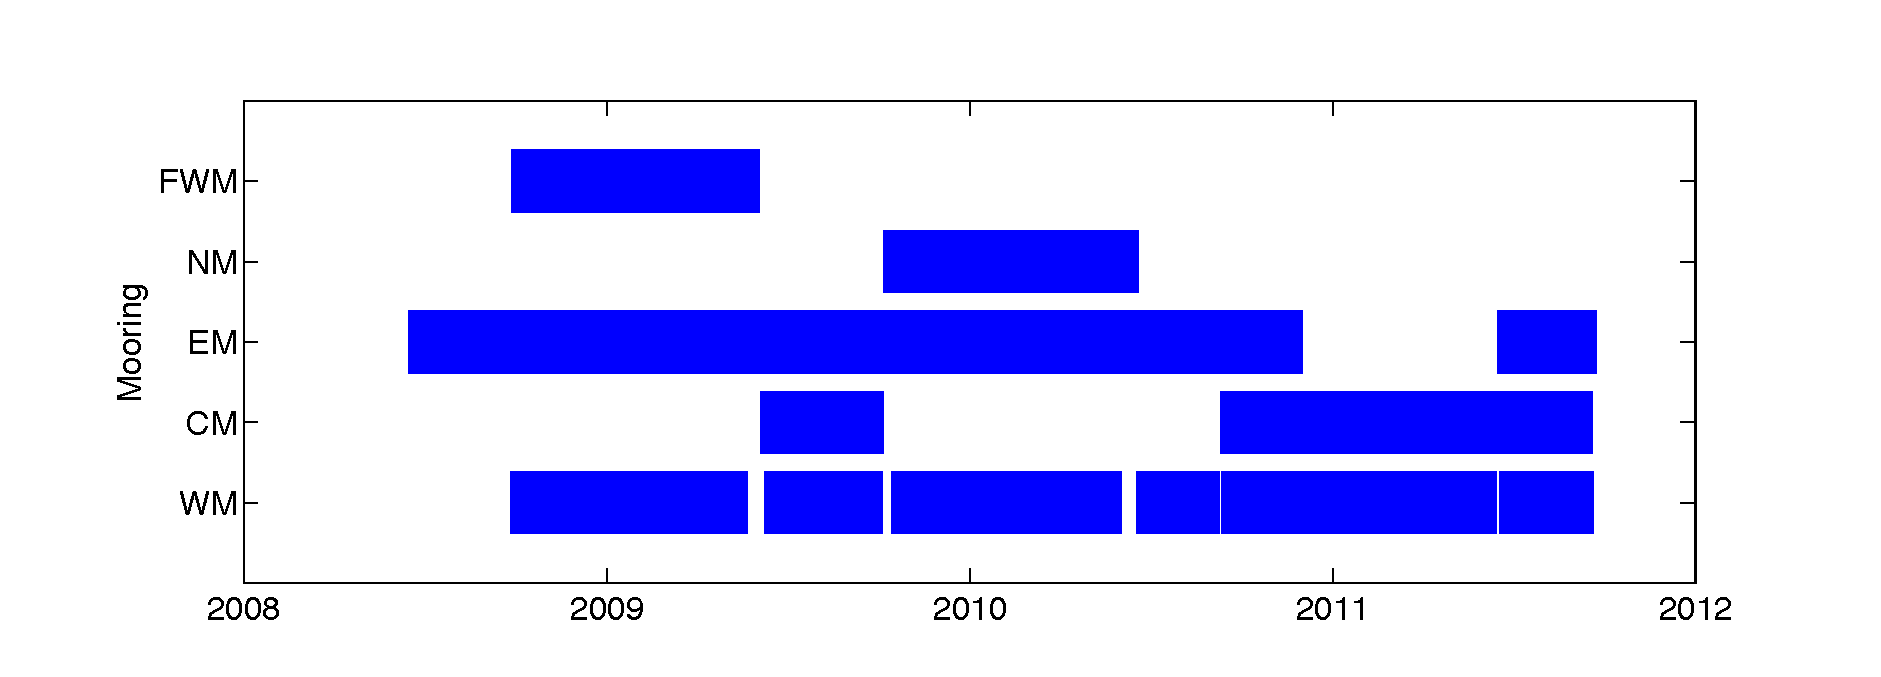
\includegraphics[height=4in]{Figures/ADCP_deployment_record.pdf}
%		\end{center}
%		\captionof{figure}{ADCP deployment record.}
%		\label{gull}
%	\end{figure}
%=============================================================================================================


%%%%%%%%%%%%%%%%%%%%%%%%%%%
% WAVELET ANALYSIS
%%%%%%%%%%%%%%%%%%%%%%%%%%%
\section{Wavelet Analysis}

Many geophysical time series have non-stationary statistics, i.e. the mean and variance change with time.
A Fourier transform can be used to determine whether a frequency is present in a time series, however, a periodogram of the Fourier transform does not give any information about 
how the amplitude of each frequency varies with time.  A simple way to deal with non-stationary time series is to compute a running variance and running mean, however,  this contains 
no frequency information and is highly dependent on the length of the window. To gain information about the frequency of a periodic signal a running
Fourier transform can be used. This involves using a certain window width and sliding it over the time series, computing the fast Fourier transform (FFT)
at each time (using only the data inside the window). The problem with the latter is that at low frequencies can not be resolved since very few, if any, oscillations will fit inside the window. Also, 
at high frequencies there are so many oscillations in the window that the frequency is not localized in time. Wavelet analysis attempts to solve this time and frequency localization
problem. 

Wavelet analyses are used to study the temporal variability of power at many different frequencies.  A wavelet is a function which has zero mean and 
is localized in time and frequency.  Traditionally, wavelets from a spectrum of frequencies are convoluted with with a time series. 
This thesis will only use wavelets tuned to a specific frequency. %inertial frequency ($\omega=\frac{2\pi}{T_i}$,  where $T_i$ is the local inertial period) will be used in this thesis.  
Time series were convoluted using a clockwise and counter-clockwise rotating Morlet wavelet of the form: 

\begin{equation}
	w_{\pm}(t_0)=(\tau \sqrt{\pi})^{-1} e^{-(\frac{(t-t_0)}{\tau})^2}e^{\mp i\omega t}
\end{equation}
where $\tau$ is window width, $\omega$ is the frequency of the wavelet, $t$ is time vector, and $t_0$ is the central position in time of the wavelet.  Power is determined using 
\begin{equation}
	P_{\pm}(t)=\int_{-\infty}^{\infty} \! w_{\pm}U \, \mathrm{d}t
\end{equation}
where $U=u+iv$ is the complex velocity ($u$ is the zonal component while $v$ is the meridional component). The power yields informations about the magnitude and phase 
of the near-inertial waves. The complex Morlet wavelet is formed from the product of a Guassian curve and a sine or cosine function, Figure ~\ref{Complex Morlet Wavelet}.

% -- MORLET WAVELET -- %
\FIGURE{3.5}{morlet.pdf}{Complex Morlet Wavelet}{Column A shows the product of a Gaussian curve and a cosine function and the column B
shows the product of a Gaussian curve and a sine function. The bottom row shows the result of these products, which are the real and complex component
of the Morlet wavelet.}


%%%%%%%%%%%%%%%%%%%%%%%%%%%
% NEAR-INERTIAL ENERGY
%%%%%%%%%%%%%%%%%%%%%%%%%%%
\section{Near-Inertial Energy}
Energy in this motion is carried in vertical oscillations of the water column, primarily at the thermocline, which represents the potential energy
or the currents associated with this motion which represents the kinetic energy. Since Lake Superior is a large Burger number lake a greater
fraction of this energy is carried in potential energy  \citep{antenucci2001energetics}. 

%=====================================================================================================================
%	NEAR INERTIAL POTENTIAL ENERGY
%=====================================================================================================================
\subsection{Near-Inertial Potential Energy}

Near-inertial potential energy is carried in undulations of pycnolines. The largest of these vertical migrations occur
at the thermocline, therefore undulations of the thermocline are commonly used as an estimate of near-inertial potential energy.
The vertical stratification scale  was estimated by the following equation:

$$z_s=\frac{\sum_{i=1}^N \frac{\Delta T_i}{\Delta z_i} z_{i,mid}}{\sum_{i=1}^N \frac{\Delta T_i}{\Delta z_i}}$$
where $z_{mid}$ is the mid point between adjacent grid cell, $\Delta T_i$ is the temperature difference of the adjacent grid cells, and $\Delta z_i$ 
is the distance between each vertical grid cell. 
 
\begin{comment}
Near-inertial potential energy is carried in undulations of pycnolines. The largest of these vertical migrations occur
at the thermocline, therefore undulations of the thermocline are commonly used as an estimate of near-inertial potential energy. Two methods
for estimating the thermocline were considered. \citet{austin2011sensitivity} proposed a method of calculating the vertical stratification scale given discrete data : 

$$z_s = \frac{\sum(T_i-T_B)\Delta z_i}{(T_S -T_B)} $$

Where $T_i$ is the temperature at depth level $i$, $T_S$ and $T_B$ are the temperature at the surface and at the bottom respectively and  $\Delta z_i$ is the spacing between observations. 
%A study in the Canadian shield lakes showed that dissolved organic carbon (DOC) concentration is the most important predictor of thermocline depth \citep{perez1999significance}. 
A common method to estimate the thermocline depth is to calculate
the maximum Brunt-V\"{a}is\"{a}l\"{a} frequency \footnote{Named in honor of Sir David Brunt and Vilho V\"{a}is\"{a}l\"{a}, the Brunt-V\"{a}is\"{a}l\"{a} frequency is also commonly referred to as buoyancy frequency} denoted by $N$ and usually written as $N^2$ : 

$$N^2 = \frac{-g}{\rho_o}\frac{\partial \rho(z)}{\partial z} $$

where $g$ is gravitational acceleration $\rho_o$ is a reference density and $\rho(z)$ is the density at depth $z$.  The depth where $N^2$ is maximum was found
to be a more robust measure the thermocline depth and will therefore be used as an estimate of the thermocline depth. 
\end{comment}

%=====================================================================================================================
%	INTEGRATED KINETIC ENERGY
%=====================================================================================================================
\subsection{Integrated Kinetic Energy}

The classical expression for kinetic energy can be used to estimate the kinetic energy of a fluid column : 

\begin{align*}
	KE &=\sum \frac{1}{2} v_i^2 \Delta m_i \\ 
	&= \frac{1}{2} \sum \rho_i A v_i^2 \Delta z_i  \\
\end{align*}

Where $m_i$ is the mass of each parcel of fluid, $v_i$ is the speed of the current at each depth $i$, $A$ is the surface area of each parcel, and $\Delta z_i$ is the thickness of 
each layer. If the surface area of each parcel is a constant then we can write the kinetic energy per area : 

$$ \frac{KE}{A} =  \frac{1}{2} \sum \rho_i v_i^2 \Delta z_i $$

Given raw velocity this expression will not tell us anything about energy at the inertial frequency. In order to establish kinetic energy at the inertial frequency a
measure for the inertial velocity needs to be established. Wavelet analysis and the rotary spectrum can be used to isolate the inertial velocity. The amplitude 
of a wavelet tuned to the inertial frequency can be used as an estimator of the inertial velocity. This method has the advantage of looking at temporal variations
of inertial energy. Another method to estimate inertial velocity is to use the rotary spectrum of the current at each depth and then pick value of the clockwise 
component at the inertial frequency. The units of this value (assuming frequency in cycles per hour) will be $m^2 s^{-2} cph^{-1}$ which is proportional to the 
inertial velocity. To transform this value into a current you need to divide by the inertial frequency and then take the square root. The latter method can be enhanced to accommodate
to a range of frequencies, in which case you would integrate under the range of frequencies and then take the square root. This method takes into account the 
entire time series and therefor you lose information about time, but this method has the advantage of defining one number for the inertial velocity. 
This thesis will use the wavelet method to estimate the inertial velocity since it provided temporal information. To speed up computation time I will assume the inertial energy
energy at the surface is representative of the total integrated kinetic energy. This can be justified since most of the kinetic energy is in the top mixed layer while weak currents
are present below the thermocline. The kinetic energy will also be weighted by the water depth at each point to take into account bathymetric effects. The expression below
was used to estimate near-inertial kinetic energy : 

$$\frac{KE}{V}=\frac{\frac{1}{2}\rho_{surf} v^2_{surf} \Delta z_{surf}}{H} $$

Where $\rho_{surf}$ is the water density at the surface, $v$ is the inertial velocity estimated from the amplitude of the clockwise wavelet at Coriolis frequency, $\Delta z_{surf}$ is the
depth at which the velocity measurement was taken, and $H$ is the water depth . 

%=================================================================================
